\documentclass[tikz]{standalone}
\usepackage{amsmath,amssymb}
\usetikzlibrary{arrows.meta}

% Classes of morphisms
\newcommand{\all}{\mathsf{all}}
\newcommand{\inj}{\mathsf{inj}}
\newcommand{\surj}{\mathsf{surj}}
\newcommand{\bij}{\mathsf{bij}}
\newcommand{\init}{\mathsf{init}}
\newcommand{\pb}{\mathsf{pb}}
\newcommand{\homog}{\mathsf{homog}}
\DeclareMathOperator{\id}{id}
\renewcommand\emptyset\varnothing
\begin{document}
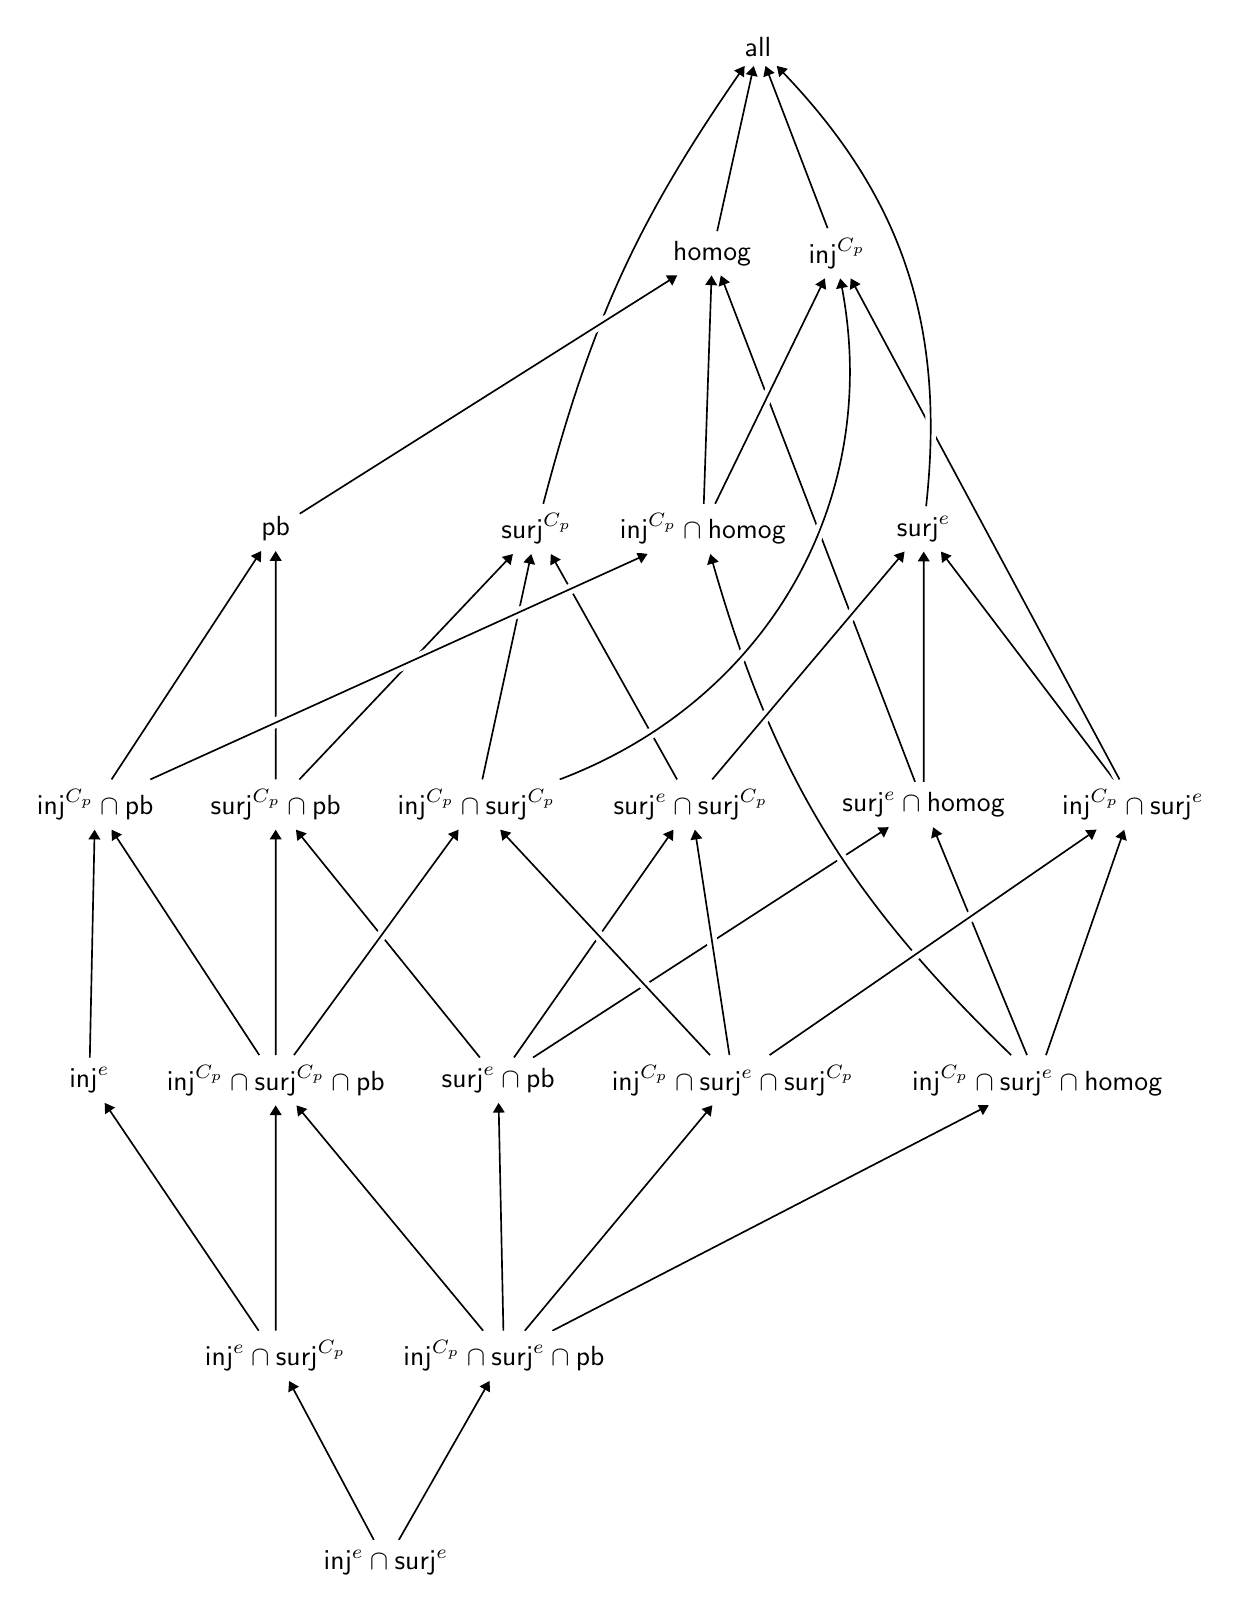
\begin{tikzpicture}[scale=3.5]
    \node (v0) at (0.5, 2.75) {$ \all $};
    \node (v1) at (0.787, 2) {$ \inj^{C_p} $};
    \node (v2) at (1.101, 1) {$ \surj^e $};
    \node (v3) at (-0.303, 1) {$ \surj^{C_p} $};
    \node (v4) at (0.334, 2) {$ \homog $};
    \node (v5) at (1.86, 0) {$ \inj^{C_p} \cap \surj^e $};
    \node (v6) at (-0.52, 0) {$ \inj^{C_p} \cap \surj^{C_p} $};
    \node (v7) at (0.3, 1) {$ \inj^{C_p} \cap \homog $};
    \node (v8) at (0.257, 0) {$ \surj^e \cap \surj^{C_p} $};
    \node (v9) at (1.101, 0) {$ \surj^e \cap \homog $};
    \node (v10) at (-1.25, 1) {$ \pb $};
    \node (v11) at (0.41, -1) {$ \inj^{C_p} \cap \surj^e \cap \surj^{C_p} $};
    \node (v12) at (1.513, -1) {$ \inj^{C_p} \cap \surj^e \cap \homog $};
    \node (v13) at (-1.905, 0) {$ \inj^{C_p} \cap \pb $};
    \node (v14) at (-1.25, 0) {$ \surj^{C_p} \cap \pb $};
    \node (v15) at (-1.926, -1) {$ \inj^e $};
    \node (v16) at (-1.25, -1) {$ \inj^{C_p} \cap \surj^{C_p} \cap \pb $};
    \node (v17) at (-0.443, -1) {$ \surj^e \cap \pb $};
    \node (v18) at (-1.25, -2) {$ \inj^e \cap \surj^{C_p} $};
    \node (v19) at (-0.422, -2) {$ \inj^{C_p} \cap \surj^e \cap \pb $};
    \node (v20) at (-0.85, -2.75) {$ \inj^e \cap \surj^e $};
    \draw[white, ultra thick, double=black, arrows={-Triangle[black,scale=0.25]}] (v20) -- (v19);
    \draw[white, ultra thick, double=black, arrows={-Triangle[black,scale=0.25]}] (v20) -- (v18);
    \draw[white, ultra thick, double=black, arrows={-Triangle[black,scale=0.25]}] (v19) -- (v17);
    \draw[white, ultra thick, double=black, arrows={-Triangle[black,scale=0.25]}] (v19) -- (v12);
    \draw[white, ultra thick, double=black, arrows={-Triangle[black,scale=0.25]}] (v19) -- (v11);
    \draw[white, ultra thick, double=black, arrows={-Triangle[black,scale=0.25]}] (v19) -- (v16);
    \draw[white, ultra thick, double=black, arrows={-Triangle[black,scale=0.25]}] (v17) -- (v9);
    \draw[white, ultra thick, double=black, arrows={-Triangle[black,scale=0.25]}] (v17) -- (v8);
    \draw[white, ultra thick, double=black, arrows={-Triangle[black,scale=0.25]}] (v17) -- (v14);
    \draw[white, ultra thick, double=black, arrows={-Triangle[black,scale=0.25]}] (v12) -- (v9);
    \draw[white, ultra thick, double=black, arrows={-Triangle[black,scale=0.25]}] (v12) -- (v5);
    \draw[white, ultra thick, double=black, arrows={-Triangle[black,scale=0.25]}] (v12) to[bend left=15] (v7);
    \draw[white, ultra thick, double=black, arrows={-Triangle[black,scale=0.25]}] (v9) -- (v2);
    \draw[white, ultra thick, double=black, arrows={-Triangle[black,scale=0.25]}] (v9) -- (v4);
    \draw[white, ultra thick, double=black, arrows={-Triangle[black,scale=0.25]}] (v11) -- (v8);
    \draw[white, ultra thick, double=black, arrows={-Triangle[black,scale=0.25]}] (v11) -- (v5);
    \draw[white, ultra thick, double=black, arrows={-Triangle[black,scale=0.25]}] (v11) -- (v6);
    \draw[white, ultra thick, double=black, arrows={-Triangle[black,scale=0.25]}] (v8) -- (v2);
    \draw[white, ultra thick, double=black, arrows={-Triangle[black,scale=0.25]}] (v8) -- (v3);
    \draw[white, ultra thick, double=black, arrows={-Triangle[black,scale=0.25]}] (v5) -- (v2);
    \draw[white, ultra thick, double=black, arrows={-Triangle[black,scale=0.25]}] (v5) -- (v1);
    \draw[white, ultra thick, double=black, arrows={-Triangle[black,scale=0.25]}] (v2) to[bend right=25] (v0);
    \draw[white, ultra thick, double=black, arrows={-Triangle[black,scale=0.25]}] (v18) -- (v16);
    \draw[white, ultra thick, double=black, arrows={-Triangle[black,scale=0.25]}] (v18) -- (v15);
    \draw[white, ultra thick, double=black, arrows={-Triangle[black,scale=0.25]}] (v16) -- (v14);
    \draw[white, ultra thick, double=black, arrows={-Triangle[black,scale=0.25]}] (v16) -- (v6);
    \draw[white, ultra thick, double=black, arrows={-Triangle[black,scale=0.25]}] (v16) -- (v13);
    \draw[white, ultra thick, double=black, arrows={-Triangle[black,scale=0.25]}] (v14) -- (v3);
    \draw[white, ultra thick, double=black, arrows={-Triangle[black,scale=0.25]}] (v14) -- (v10);
    \draw[white, ultra thick, double=black, arrows={-Triangle[black,scale=0.25]}] (v6) -- (v3);
    \draw[white, ultra thick, double=black, arrows={-Triangle[black,scale=0.25]}] (v6) to[bend right=40] (v1);
    \draw[white, ultra thick, double=black, arrows={-Triangle[black,scale=0.25]}] (v3) to[bend left=10] (v0);
    \draw[white, ultra thick, double=black, arrows={-Triangle[black,scale=0.25]}] (v15) -- (v13);
    \draw[white, ultra thick, double=black, arrows={-Triangle[black,scale=0.25]}] (v13) -- (v10);
    \draw[white, ultra thick, double=black, arrows={-Triangle[black,scale=0.25]}] (v13) -- (v7);
    \draw[white, ultra thick, double=black, arrows={-Triangle[black,scale=0.25]}] (v10) -- (v4);
    \draw[white, ultra thick, double=black, arrows={-Triangle[black,scale=0.25]}] (v7) -- (v4);
    \draw[white, ultra thick, double=black, arrows={-Triangle[black,scale=0.25]}] (v7) -- (v1);
    \draw[white, ultra thick, double=black, arrows={-Triangle[black,scale=0.25]}] (v4) -- (v0);
    \draw[white, ultra thick, double=black, arrows={-Triangle[black,scale=0.25]}] (v1) -- (v0);
    \node[fill=white] at (v0) {$ \all $};
    \node[fill=white] at (v1) {$ \inj^{C_p} $};
    \node[fill=white] at (v2) {$ \surj^e $};
    \node[fill=white] at (v3) {$ \surj^{C_p} $};
    \node[fill=white] at (v4) {$ \homog $};
    \node[fill=white] at (v5) {$ \inj^{C_p} \cap \surj^e $};
    \node[fill=white] at (v6) {$ \inj^{C_p} \cap \surj^{C_p} $};
    \node[fill=white] at (v7) {$ \inj^{C_p} \cap \homog $};
    \node[fill=white] at (v8) {$ \surj^e \cap \surj^{C_p} $};
    \node[fill=white] at (v9) {$ \surj^e \cap \homog $};
    \node[fill=white] at (v10) {$ \pb $};
    \node[fill=white] at (v11) {$ \inj^{C_p} \cap \surj^e \cap \surj^{C_p} $};
    \node[fill=white] at (v12) {$ \inj^{C_p} \cap \surj^e \cap \homog $};
    \node[fill=white] at (v13) {$ \inj^{C_p} \cap \pb $};
    \node[fill=white] at (v14) {$ \surj^{C_p} \cap \pb $};
    \node[fill=white] at (v15) {$ \inj^e $};
    \node[fill=white] at (v16) {$ \inj^{C_p} \cap \surj^{C_p} \cap \pb $};
    \node[fill=white] at (v17) {$ \surj^e \cap \pb $};
    \node[fill=white] at (v18) {$ \inj^e \cap \surj^{C_p} $};
    \node[fill=white] at (v19) {$ \inj^{C_p} \cap \surj^e \cap \pb $};
    \node[fill=white] at (v20) {$ \inj^e \cap \surj^e $};
\end{tikzpicture}
\end{document}

